\documentclass{standalone}
\usepackage{tikz}
\usetikzlibrary{patterns, positioning}

\begin{document}
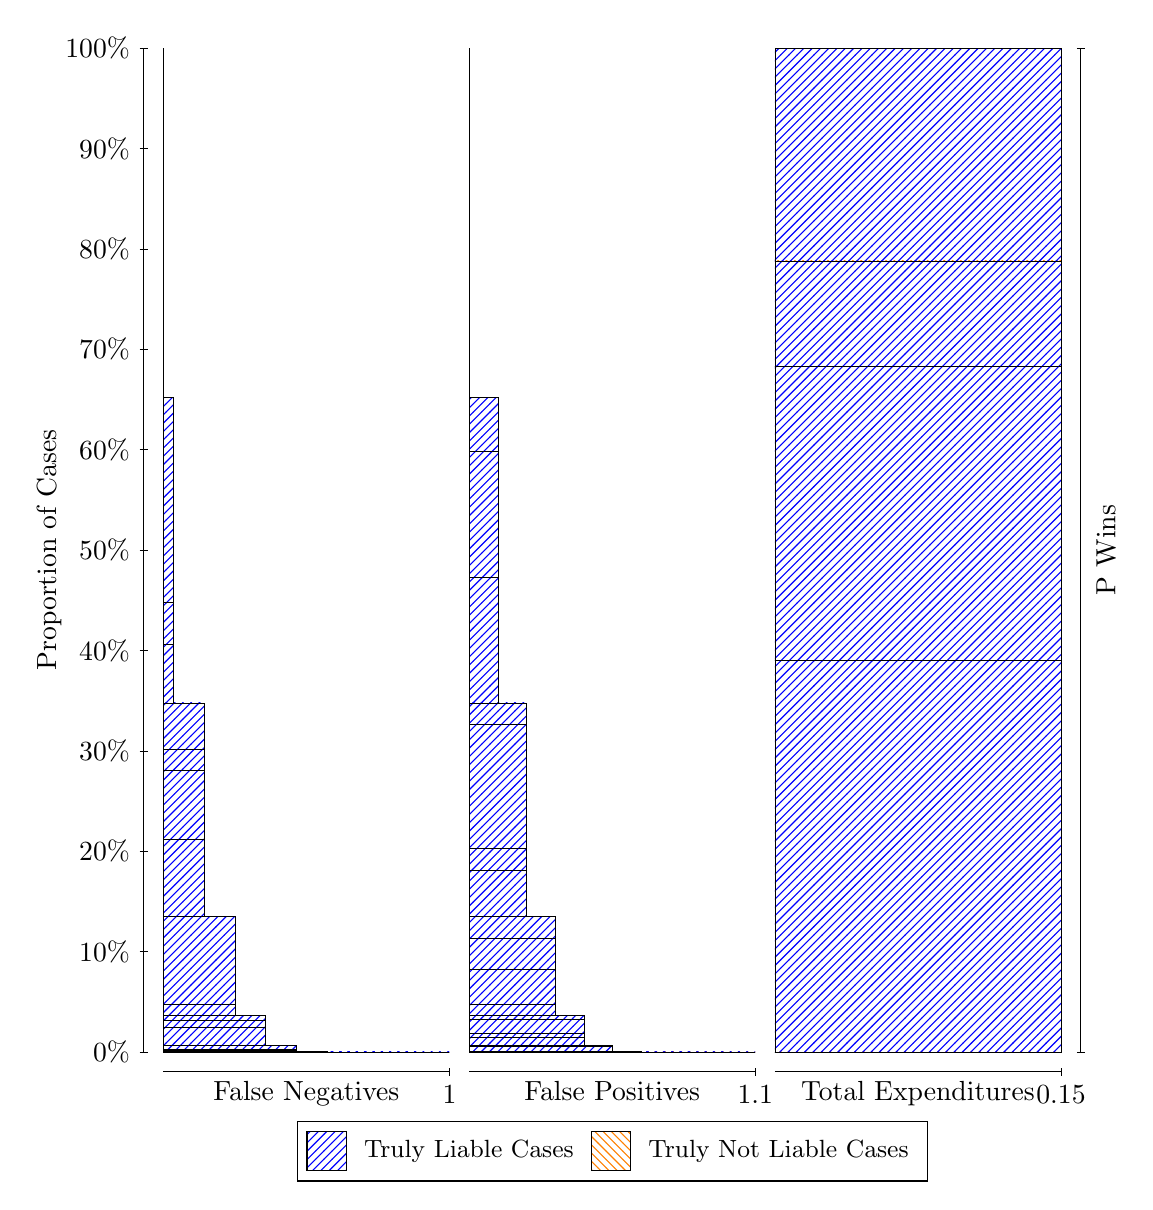
\begin{tikzpicture}
\draw[black, very thin] (1.5,1.75) -- (1.5,14.5);
\node[rotate=90, anchor=center] at (0.3, 8.125) {Proportion of Cases};
\draw[black, very thin] (1.45,1.75) -- (1.55,1.75);
\node[anchor=east] at (1.45, 1.75) {0\%};
\draw[black, very thin] (1.45,3.025) -- (1.55,3.025);
\node[anchor=east] at (1.45, 3.025) {10\%};
\draw[black, very thin] (1.45,4.3) -- (1.55,4.3);
\node[anchor=east] at (1.45, 4.3) {20\%};
\draw[black, very thin] (1.45,5.575) -- (1.55,5.575);
\node[anchor=east] at (1.45, 5.575) {30\%};
\draw[black, very thin] (1.45,6.85) -- (1.55,6.85);
\node[anchor=east] at (1.45, 6.85) {40\%};
\draw[black, very thin] (1.45,8.125) -- (1.55,8.125);
\node[anchor=east] at (1.45, 8.125) {50\%};
\draw[black, very thin] (1.45,9.4) -- (1.55,9.4);
\node[anchor=east] at (1.45, 9.4) {60\%};
\draw[black, very thin] (1.45,10.675) -- (1.55,10.675);
\node[anchor=east] at (1.45, 10.675) {70\%};
\draw[black, very thin] (1.45,11.95) -- (1.55,11.95);
\node[anchor=east] at (1.45, 11.95) {80\%};
\draw[black, very thin] (1.45,13.225) -- (1.55,13.225);
\node[anchor=east] at (1.45, 13.225) {90\%};
\draw[black, very thin] (1.45,14.5) -- (1.55,14.5);
\node[anchor=east] at (1.45, 14.5) {100\%};

\draw[black, very thin] (13.4,1.75) -- (13.4,14.5);
\draw[black, very thin] (13.35,1.75) -- (13.45,1.75);
\node[anchor=west] at (13.35, 1.75) {};
\draw[black, very thin] (13.35,14.5) -- (13.45,14.5);
\node[anchor=west] at (13.35, 14.5) {};

\draw[black, very thin, pattern color=blue, pattern=north east lines] (1.75,1.75) rectangle (5.3833,1.75);
\draw[black, very thin, pattern color=blue, pattern=north east lines] (1.75,1.75) rectangle (4.9942,1.75);
\draw[black, very thin, pattern color=blue, pattern=north east lines] (1.75,1.75) rectangle (4.9942,1.75);
\draw[black, very thin, pattern color=blue, pattern=north east lines] (1.75,1.75) rectangle (4.6051,1.75);
\draw[black, very thin, pattern color=blue, pattern=north east lines] (1.75,1.75) rectangle (4.216,1.7502);
\draw[black, very thin, pattern color=blue, pattern=north east lines] (1.75,1.7502) rectangle (4.216,1.7507);
\draw[black, very thin, pattern color=blue, pattern=north east lines] (1.75,1.7507) rectangle (3.8269,1.758);
\draw[black, very thin, pattern color=blue, pattern=north east lines] (1.75,1.758) rectangle (3.8269,1.7599);
\draw[black, very thin, pattern color=blue, pattern=north east lines] (1.75,1.7599) rectangle (3.4378,1.7707);
\draw[black, very thin, pattern color=blue, pattern=north east lines] (1.75,1.7707) rectangle (3.4378,1.782);
\draw[black, very thin, pattern color=blue, pattern=north east lines] (1.75,1.782) rectangle (3.4378,1.8337);
\draw[black, very thin, pattern color=blue, pattern=north east lines] (1.75,1.8337) rectangle (3.0487,2.0583);
\draw[black, very thin, pattern color=blue, pattern=north east lines] (1.75,2.0583) rectangle (3.0487,2.1561);
\draw[black, very thin, pattern color=blue, pattern=north east lines] (1.75,2.1561) rectangle (3.0487,2.2136);
\draw[black, very thin, pattern color=blue, pattern=north east lines] (1.75,2.2136) rectangle (2.6595,2.3552);
\draw[black, very thin, pattern color=blue, pattern=north east lines] (1.75,2.3552) rectangle (2.6595,3.4713);
\draw[black, very thin, pattern color=blue, pattern=north east lines] (1.75,3.4713) rectangle (2.2704,4.449);
\draw[black, very thin, pattern color=blue, pattern=north east lines] (1.75,4.449) rectangle (2.2704,5.322);
\draw[black, very thin, pattern color=blue, pattern=north east lines] (1.75,5.322) rectangle (2.2704,5.5912);
\draw[black, very thin, pattern color=blue, pattern=north east lines] (1.75,5.5912) rectangle (2.2704,6.182);
\draw[black, very thin, pattern color=blue, pattern=north east lines] (1.75,6.182) rectangle (1.8813,6.9274);
\draw[black, very thin, pattern color=blue, pattern=north east lines] (1.75,6.9274) rectangle (1.8813,7.4554);
\draw[black, very thin, pattern color=blue, pattern=north east lines] (1.75,7.4554) rectangle (1.8813,10.068);
\draw[black, very thin, pattern color=orange, pattern=north west lines] (1.75,10.068) rectangle (1.75,10.068);
\draw[black, very thin, pattern color=blue, pattern=north east lines] (1.75,10.068) rectangle (1.75,14.5);
\draw[black, very thin, pattern color=orange, pattern=north west lines] (5.6333,1.75) rectangle (9.2667,1.75);
\draw[black, very thin, pattern color=blue, pattern=north east lines] (5.6333,1.75) rectangle (9.2667,1.75);
\draw[black, very thin, pattern color=orange, pattern=north west lines] (5.6333,1.75) rectangle (8.9038,1.75);
\draw[black, very thin, pattern color=blue, pattern=north east lines] (5.6333,1.75) rectangle (8.9038,1.75);
\draw[black, very thin, pattern color=blue, pattern=north east lines] (5.6333,1.75) rectangle (8.5409,1.75);
\draw[black, very thin, pattern color=orange, pattern=north west lines] (5.6333,1.75) rectangle (8.5409,1.75);
\draw[black, very thin, pattern color=blue, pattern=north east lines] (5.6333,1.75) rectangle (8.5409,1.75);
\draw[black, very thin, pattern color=blue, pattern=north east lines] (5.6333,1.75) rectangle (8.178,1.7502);
\draw[black, very thin, pattern color=blue, pattern=north east lines] (5.6333,1.7502) rectangle (8.178,1.7503);
\draw[black, very thin, pattern color=orange, pattern=north west lines] (5.6333,1.7503) rectangle (8.178,1.7503);
\draw[black, very thin, pattern color=blue, pattern=north east lines] (5.6333,1.7503) rectangle (8.178,1.7507);
\draw[black, very thin, pattern color=orange, pattern=north west lines] (5.6333,1.7507) rectangle (7.8151,1.7507);
\draw[black, very thin, pattern color=blue, pattern=north east lines] (5.6333,1.7507) rectangle (7.8151,1.7564);
\draw[black, very thin, pattern color=blue, pattern=north east lines] (5.6333,1.7564) rectangle (7.8151,1.758);
\draw[black, very thin, pattern color=blue, pattern=north east lines] (5.6333,1.758) rectangle (7.8151,1.7599);
\draw[black, very thin, pattern color=orange, pattern=north west lines] (5.6333,1.7599) rectangle (7.4523,1.7599);
\draw[black, very thin, pattern color=blue, pattern=north east lines] (5.6333,1.7599) rectangle (7.4523,1.8223);
\draw[black, very thin, pattern color=blue, pattern=north east lines] (5.6333,1.8223) rectangle (7.4523,1.8337);
\draw[black, very thin, pattern color=blue, pattern=north east lines] (5.6333,1.8337) rectangle (7.0894,1.9334);
\draw[black, very thin, pattern color=blue, pattern=north east lines] (5.6333,1.9334) rectangle (7.0894,1.991);
\draw[black, very thin, pattern color=orange, pattern=north west lines] (5.6333,1.991) rectangle (7.0894,1.991);
\draw[black, very thin, pattern color=blue, pattern=north east lines] (5.6333,1.991) rectangle (7.0894,2.1647);
\draw[black, very thin, pattern color=blue, pattern=north east lines] (5.6333,2.1647) rectangle (7.0894,2.2136);
\draw[black, very thin, pattern color=blue, pattern=north east lines] (5.6333,2.2136) rectangle (6.7265,2.3564);
\draw[black, very thin, pattern color=blue, pattern=north east lines] (5.6333,2.3564) rectangle (6.7265,2.796);
\draw[black, very thin, pattern color=orange, pattern=north west lines] (5.6333,2.796) rectangle (6.7265,2.796);
\draw[black, very thin, pattern color=blue, pattern=north east lines] (5.6333,2.796) rectangle (6.7265,3.1882);
\draw[black, very thin, pattern color=blue, pattern=north east lines] (5.6333,3.1882) rectangle (6.7265,3.4713);
\draw[black, very thin, pattern color=blue, pattern=north east lines] (5.6333,3.4713) rectangle (6.3636,4.0599);
\draw[black, very thin, pattern color=blue, pattern=north east lines] (5.6333,4.0599) rectangle (6.3636,4.3313);
\draw[black, very thin, pattern color=orange, pattern=north west lines] (5.6333,4.3313) rectangle (6.3636,4.3313);
\draw[black, very thin, pattern color=blue, pattern=north east lines] (5.6333,4.3313) rectangle (6.3636,5.9129);
\draw[black, very thin, pattern color=blue, pattern=north east lines] (5.6333,5.9129) rectangle (6.3636,6.182);
\draw[black, very thin, pattern color=blue, pattern=north east lines] (5.6333,6.182) rectangle (6.0007,7.7726);
\draw[black, very thin, pattern color=orange, pattern=north west lines] (5.6333,7.7726) rectangle (6.0007,7.7726);
\draw[black, very thin, pattern color=blue, pattern=north east lines] (5.6333,7.7726) rectangle (6.0007,9.3821);
\draw[black, very thin, pattern color=blue, pattern=north east lines] (5.6333,9.3821) rectangle (6.0007,10.068);
\draw[black, very thin, pattern color=blue, pattern=north east lines] (5.6333,10.068) rectangle (5.6379,10.339);
\draw[black, very thin, pattern color=blue, pattern=north east lines] (5.6333,10.339) rectangle (5.6379,12.496);
\draw[black, very thin, pattern color=blue, pattern=north east lines] (5.6333,12.496) rectangle (5.6379,12.779);
\draw[black, very thin, pattern color=blue, pattern=north east lines] (5.6333,12.779) rectangle (5.6333,14.5);
\draw[black, very thin, pattern color=orange, pattern=north west lines] (9.5167,1.75) rectangle (13.15,1.75);
\draw[black, very thin, pattern color=blue, pattern=north east lines] (9.5167,1.75) rectangle (13.15,6.7273);
\draw[black, very thin, pattern color=orange, pattern=north west lines] (9.5167,6.7273) rectangle (13.15,6.7273);
\draw[black, very thin, pattern color=blue, pattern=north east lines] (9.5167,6.7273) rectangle (13.15,10.46);
\draw[black, very thin, pattern color=orange, pattern=north west lines] (9.5167,10.46) rectangle (13.15,10.46);
\draw[black, very thin, pattern color=blue, pattern=north east lines] (9.5167,10.46) rectangle (13.15,11.796);
\draw[black, very thin, pattern color=orange, pattern=north west lines] (9.5167,11.796) rectangle (13.15,11.796);
\draw[black, very thin, pattern color=blue, pattern=north east lines] (9.5167,11.796) rectangle (13.15,14.5);
\draw[black, very thin] (1.75,1.5) -- (5.3833,1.5);
\node[anchor=north] at (3.5667, 1.5) {False Negatives};
\draw[black, very thin] (5.3833,1.45) -- (5.3833,1.55);
\node[anchor=north] at (5.3833, 1.45) {1};

\draw[black, very thin] (5.6333,1.5) -- (9.2667,1.5);
\node[anchor=north] at (7.45, 1.5) {False Positives};
\draw[black, very thin] (9.2667,1.45) -- (9.2667,1.55);
\node[anchor=north] at (9.2667, 1.45) {1.1};

\draw[black, very thin] (9.5167,1.5) -- (13.15,1.5);
\node[anchor=north] at (11.333, 1.5) {Total Expenditures};
\draw[black, very thin] (13.15,1.45) -- (13.15,1.55);
\node[anchor=north] at (13.15, 1.45) {0.15};

\node[black, centered, rotate=90] at (13.72, 8.125) {P Wins};

\draw (7.449999999999999,1.5) node[draw=none] (baseCoordinate) {};
\begin{scope}[align=center]
        \matrix[scale=0.5, draw=black, below=0.5cm of baseCoordinate, nodes={draw}, column sep=0.1cm]{
            \node[rectangle, draw, minimum width=0.5cm, minimum height=0.5cm, pattern=north east lines, pattern color=blue] {}; &
            \node[draw=none, font=\small] (B) {Truly Liable Cases}; &
            \node[rectangle, draw, minimum width=0.5cm, minimum height=0.5cm, pattern=north west lines, pattern color=orange] {}; &
            \node[draw=none, font=\small] (B) {Truly Not Liable Cases}; \\
            };
\end{scope}

\end{tikzpicture}
\end{document}